% QAI 2026 talk: Measurement-Efficient DQAS (arXiv:2610.10351)
% Storyline: "Audit Your Bill" (MaxCut -> Hook -> Parameter-Shift -> Diagonal H & Commutation / Cases 1-2 -> DQAS -> ME-DQAS -> Results)
% Build: pdflatex main.tex && pdflatex main.tex   (or lualatex for WorkSans)
% Speaker notes: \note{...} below each frame. To see them, uncomment
% \setbeameroption{show notes on second screen=right}
\documentclass[aspectratio=169,10pt]{beamer}
\usepackage{lamarrtheme} % Lamarr look (inofficial template); build with lualatex or pdflatex
% \setbeameroption{show notes on second screen=right}
\usepackage[T1]{fontenc}
\usepackage{amsmath,amssymb,braket}
\usepackage{booktabs}
\usepackage{graphicx}
\usepackage{tikz}
\usetikzlibrary{positioning,arrows.meta,calc,shapes.geometric,decorations.pathreplacing,fit}
\usepackage{pgfplots}
\pgfplotsset{compat=1.16}
\usepackage{qrcode}
\graphicspath{{figures/}{../dataset/}}

% talk colours mapped onto the Lamarr palette
\colorlet{base}{softgray}
\colorlet{me}{aqua}
\colorlet{zero}{carribean}
\colorlet{one}{sunshine}
\colorlet{warn}{fuchsia}

\newcommand{\refs}[1]{{\scriptsize\color{gray}[#1]}}

% tiny circuit helpers
\tikzset{
  wire/.style={draw=black!70, line width=0.6pt},
  gate/.style={draw, fill=white, minimum width=0.85cm, minimum height=0.6cm, inner sep=1pt, font=\small},
  hl/.style={gate, fill=me!15, draw=me, line width=1pt},
  zg/.style={gate, fill=zero!15, draw=zero, line width=1pt},
  meter/.style={draw, fill=white, minimum width=0.7cm, minimum height=0.6cm},
}
\newcommand{\meter}[1]{%
  \begin{scope}[shift={#1}]
    \draw[fill=white] (-0.35,-0.3) rectangle (0.35,0.3);
    \draw (-0.22,-0.15) arc (160:20:0.235);
    \draw[-{Stealth[length=3pt]}] (0,-0.2) -- ++(55:0.4);
  \end{scope}}

\title[Do you really need to measure that gradient?]{Do you really need to measure that gradient?}
\subtitle{Measurement-Efficient Differentiable Quantum Architecture Search for Combinatorial Optimization}
\author[Theißinger, Gerlach, Bauckhage]{Lukas Theißinger \quad Thore Gerlach \quad Christian Bauckhage}
\date{Univ.\ Bonn \textperiodcentered\ ESA \textperiodcentered\ Lamarr Institute \quad QAI 2026, Nottingham}

\begin{document}

% ---------------------------------------------------------------- 0 title
\maketitleframe
\note{
[0:00, 20 s; 15 min talk + 5 min Q\&A] Hi everyone—2pm on the last day, I promise no 20-line proofs, just a quick receipt audit of where quantum shots actually go when training variational circuits, and an exact way to cut about 40\% of them before touching hardware.
}

% ---------------------------------------------------------------- 1 setup: textbook MaxCut starting point
\begin{frame}{MaxCut on a quantum computer}
  \centering
  \vspace{2mm}
  \begin{tikzpicture}[scale=0.95, transform shape,
      v0/.style={circle, draw=me, fill=me!20, line width=1pt, minimum size=0.58cm, inner sep=0pt, font=\small\bfseries},
      v1/.style={circle, draw=one!85!black, fill=one!30, line width=1pt, minimum size=0.58cm, inner sep=0pt, font=\small\bfseries}]
    % Left: small 4-node MaxCut graph
    \node[v0] (n1) at (0.0, 1.35) {$0$};
    \node[v1] (n2) at (1.5, 1.35) {$1$};
    \node[v0] (n3) at (0.0, 0.00) {$0$};
    \node[v1] (n4) at (1.5, 0.00) {$1$};
    \draw[black!75, line width=0.9pt] (n1) -- (n2) -- (n4) -- (n3) -- (n1);
    \draw[black!75, line width=0.9pt] (n2) -- (n3);
    % Dashed cut line separating {n1,n3}=0 from {n2,n4}=1
    \draw[warn, dashed, line width=1pt] (0.75, 1.75) -- (0.75, -0.40);
    \node[font=\small\bfseries, align=center] at (0.75, -0.82) {1.\ MaxCut problem};
    \node[font=\scriptsize, color=gray, align=center] at (0.75, -1.18) {split nodes into $\{0,1\}$};

    % Arrow 1 -> 2
    \draw[-{Stealth}, thick, black!70] (2.15, 0.68) -- (2.95, 0.68);

    % Middle: small parameterized quantum circuit
    \begin{scope}[shift={(3.25, -0.12)}]
      \foreach \y in {0, 0.52, 1.04, 1.56} \draw[wire] (0,\y) -- (3.35,\y);
      \node[gate, minimum width=0.72cm, minimum height=0.42cm, font=\scriptsize] at (0.75, 1.56) {$R_y(\theta_1)$};
      \node[gate, minimum width=0.72cm, minimum height=0.42cm, font=\scriptsize] at (0.75, 0.52) {$R_x(\theta_2)$};
      \fill (1.65, 1.56) circle (1.8pt); \fill (1.65, 1.04) circle (1.8pt); \draw (1.65, 1.04) -- (1.65, 1.56);
      \fill (1.95, 0.52) circle (1.8pt); \fill (1.95, 0.00) circle (1.8pt); \draw (1.95, 0.00) -- (1.95, 0.52);
      \node[gate, minimum width=0.72cm, minimum height=0.42cm, font=\scriptsize] at (2.65, 1.04) {$R_z(\theta_3)$};
      \node[gate, minimum width=0.72cm, minimum height=0.42cm, font=\scriptsize] at (2.65, 0.00) {$R_y(\theta_4)$};
      \foreach \y in {0, 0.52, 1.04, 1.56} {
        \begin{scope}[shift={(3.60, \y)}, scale=0.68]
          \draw[fill=white] (-0.35,-0.3) rectangle (0.35,0.3);
          \draw (-0.22,-0.15) arc (160:20:0.235);
          \draw[-{Stealth[length=2.5pt]}] (0,-0.2) -- ++(55:0.4);
        \end{scope}
      }
      \node[font=\small\bfseries, align=center] at (1.85, -0.70) {2.\ Parameterized circuit};
      \node[font=\scriptsize, color=gray, align=center] at (1.85, -1.06) {unitaries $U(\theta)$ + readout};
    \end{scope}

    % Arrow 2 -> 3
    \draw[-{Stealth}, thick, black!70] (7.45, 0.68) -- (8.25, 0.68);

    % Right: bit strings & update loop
    \node[draw=me, fill=me!10, rounded corners, minimum width=2.45cm, minimum height=1.55cm, align=center, font=\small] (out) at (9.65, 0.68)
      {\texttt{0110}, \texttt{1001}, \dots\\[3pt]\scriptsize score cuts \&\\[1pt]\scriptsize update angles $\theta$};
    \node[font=\small\bfseries, align=center] at (9.65, -0.82) {3.\ Classical optimizer};
    \node[font=\scriptsize, color=gray, align=center] at (9.65, -1.18) {repeat until good cuts};
    \draw[-{Stealth[length=5.5pt]}, thick, me, rounded corners=4pt]
      (out.north) -- (9.65, 2.25) -- (5.10, 2.25) node[midway, above=2pt, font=\scriptsize\bfseries, text=me] {update $\theta$} -- (5.10, 1.75);
  \end{tikzpicture}
\end{frame}
\note{
[0:20, 45 s] To get started, take a textbook example: solving MaxCut on a quantum computer.
Map each node to a qubit, apply a fixed parameterized circuit $U(\theta)$, measure bit strings to score cuts, and update the angles $\theta$ with a classical optimizer.
Simple recipe—so I ran it, and realized updating the parameters ate a shocking number of measurements.
}

% ---------------------------------------------------------------- 2 spoiler: where do the measurements go?
\begin{frame}{Where the measurements actually go}
  \centering
  \vspace{-2.5mm}
  \begin{tikzpicture}
    % Top bar: total quantum computer runs (12.70 cm = 100%)
    % 7.4% solution quality = 0.94 cm; 92.6% estimating gradients = 11.76 cm
    \node[anchor=west, font=\normalsize\bfseries, text=navy] at (0, 4.02)
      {Total measurements spent {\small\normalfont\color{softgray}(training circuits for MaxCut / 3-SAT)}};

    \fill[navy!14] (0.00, 2.82) rectangle (0.94, 3.74);
    \draw[navy!35, line width=0.5pt] (0.00, 2.82) rectangle (0.94, 3.74);
    \fill[navy!90] (0.94, 2.82) rectangle (12.70, 3.74);
    \draw[white, line width=1.4pt] (0.94, 2.82) -- (0.94, 3.74);

    \node[font=\normalsize\bfseries, text=navy] at (0.47, 3.28) {7\%};
    \node[anchor=east, font=\small, align=right, text=navy!75] at (-0.14, 3.28) {solution\\[-1pt]quality};
    \node[font=\large\bfseries, text=white] at (6.82, 3.28) {$\sim$93\% spent estimating gradients};

    % Zoom connector & breakdown of gradient measurements
    \uncover<2->{
      \fill[navy!6] (0.94, 2.82) -- (12.70, 2.82) -- (12.70, 1.92) -- (0.00, 1.92) -- cycle;
      \draw[navy!40, dashed, line width=0.9pt] (0.94, 2.82) -- (0.00, 1.92);
      \draw[navy!40, dashed, line width=0.9pt] (12.70, 2.82) -- (12.70, 1.92);

      \node[font=\normalsize\bfseries, text=navy] at (6.35, 2.37) {Looking closer at those gradient measurements:};

      % Bottom bar: 100% of gradient runs = 12.70 cm
      % 59.6% needed = 7.57 cm; 8.2% redundant = 1.04 cm; 32.2% zero = 4.09 cm
      \fill[navy!58]   (0.00, 0.90) rectangle (7.57, 1.92);
      \fill[sunshine]  (7.57, 0.90) rectangle (8.61, 1.92);
      \fill[indianred] (8.61, 0.90) rectangle (12.70, 1.92);
      \draw[white, line width=1.4pt] (7.57, 0.90) -- (7.57, 1.92);
      \draw[white, line width=1.4pt] (8.61, 0.90) -- (8.61, 1.92);

      \node[font=\large\bfseries, text=white] at (3.785, 1.41) {$\sim$60\% necessary};
      \node[font=\normalsize\bfseries, text=navy] at (8.09, 1.41) {$\sim$8\%};
      \node[font=\large\bfseries, text=white] at (10.655, 1.41) {$\sim$32\% exact ZERO};

      % Labels under bottom bar
      \draw[sunshine!70!black, line width=0.9pt] (8.09, 0.90) -- (8.09, 0.62);
      \node[below, font=\small, align=center, text=sunshine!65!black] at (8.09, 0.62)
        {\textbf{redundant}\\[-1pt]{\footnotesize\color{navy!80}(measured twice)}};
      \draw[indianred!90!black, line width=0.9pt] (10.80, 0.90) -- (10.80, 0.62);
      \node[below, font=\small, align=center, text=indianred!85!black] at (10.80, 0.62)
        {\textbf{measuring pure noise}\\[-1pt]{\footnotesize(0 runs needed)}};
    }

    \uncover<3->{
      \draw[decorate, decoration={brace, amplitude=6pt, mirror}, me, line width=1.4pt]
        (7.57, -0.34) -- (12.70, -0.34)
        node[midway, below=5pt, font=\normalsize\bfseries, text=me] {$\approx$\,40\% saved};
    }
  \end{tikzpicture}

  \vspace{1mm}
  \uncover<3->{%
    {\large We catch \textcolor{me}{\textbf{$\approx$40\%}} \textbf{classically} before running hardware,\\[-1pt]
    \textbf{without quality loss} in the gradient.}%
  }
\end{frame}
\note{
[1:05, 1:00] (5 s hand-raise bet before clicking: "What fraction of that 93\% do you think is provably ZERO?")
As you can see here, calculating the quality of a solution made up only 7\% of all measurements spent,
while 93\% went into estimating the gradients!
(click) Well, first I asked myself: why is that? Can we save some of this spending?
Analyzing the gradient calculations closer, I found that 60\% were actually necessary, while 8\% were
redundant and 32\% were \emph{exactly zero}.
(click) We catch about 40\% classically before running hardware, without quality loss in the gradient.
So let's walk through this in order: first, why do gradients eat 93\% of the bill? Second, how can we
beat that cost classically? And finally, where does this happen at scale in quantum architecture search?
}

% ---------------------------------------------------------------- 3 gradient formulas: parameter-shift vs commutator
\begin{frame}{Gradient formulas}
  \centering
  \vspace{-3mm}
  % ---- 1. Parameter-shift rule (gold standard) ----
  \begin{tikzpicture}[
      eqpart/.style={inner sep=1.4pt, outer sep=0pt, font=\large},
      term/.style={eqpart, rounded corners=2.5pt, inner xsep=3pt, inner ysep=1.5pt}]
    \node[anchor=west, font=\normalsize\bfseries, text=navy] (lbl1) at (-6.2, 1.38)
      {1.\ Parameter-shift rule {\small\normalfont\color{softgray}(gold standard)}};

    \node[eqpart] (lhs) at (-2.35, 0.20) {$\displaystyle \frac{\partial F}{\partial\theta_j} = \frac{1}{2}\Big[$};
    \node[term, right=1pt of lhs] (fp) {$\displaystyle F\!\big(\theta_j + \tfrac{\pi}{2}\big)$};
    \node[eqpart, right=1pt of fp] (mi) {$\displaystyle -$};
    \node[term, right=1pt of mi] (fm) {$\displaystyle F\!\big(\theta_j - \tfrac{\pi}{2}\big)$};
    \node[eqpart, right=1pt of fm] (rhs) {$\displaystyle \Big]$};

    \node[draw=navy!75, fill=navy!4, rounded corners=4pt, line width=1pt,
          inner xsep=9pt, inner ysep=4pt, fit=(lhs)(fp)(mi)(fm)(rhs)] (eqbox) {};
    \node[eqpart] at (lhs) {$\displaystyle \frac{\partial F}{\partial\theta_j} = \frac{1}{2}\Big[$};
    \node[eqpart] at (mi) {$\displaystyle -$};
    \node[eqpart] at (rhs) {$\displaystyle \Big]$};
    \only<1>{
      \node[term] at (fp) {$\displaystyle F\!\big(\theta_j + \tfrac{\pi}{2}\big)$};
      \node[term] at (fm) {$\displaystyle F\!\big(\theta_j - \tfrac{\pi}{2}\big)$};
    }
    \only<2->{
      \node[term, fill=warn!12, draw=warn!55, line width=0.6pt] at (fp) {$\displaystyle F\!\big(\theta_j + \tfrac{\pi}{2}\big)$};
      \node[term, fill=warn!12, draw=warn!55, line width=0.6pt] at (fm) {$\displaystyle F\!\big(\theta_j - \tfrac{\pi}{2}\big)$};
    }
    \node[anchor=south east, font=\scriptsize, text=gray, inner sep=1pt] at ([yshift=1.5pt]eqbox.north east)
      {\refs{Mitarai+ 2018; Schuld+ 2019}};

    \uncover<2->{
      \node[font=\normalsize, text=warn, inner sep=1.5pt] (two) at ($(fp.south)!0.5!(fm.south) + (0, -0.78)$)
        {\textbf{2 shifted circuits per angle}};
      \node[font=\normalsize, anchor=east, inner sep=1.5pt] at ([xshift=-7pt]two.west)
        {\textbf{1} circuit for $F(\theta)$ \;\; vs.};
      \draw[-{Stealth[length=5pt]}, warn, line width=1.05pt]
        (fp.south) to[out=-90, in=105] ([xshift=-12pt]two.north);
      \draw[-{Stealth[length=5pt]}, warn, line width=1.05pt]
        (fm.south) to[out=-90, in=75] ([xshift=12pt]two.north);
    }
  \end{tikzpicture}

  \vspace{1.5mm}
  % ---- 2. Commutator rule (also exact, less known) ----
  \uncover<3->{%
    \begin{tikzpicture}
      \node[anchor=west, font=\normalsize\bfseries, text=me] (lbl2) at (-6.2, 1.56)
        {Is parameter shift the only exact way? \;No — 2.\ Commutator rule {\small\normalfont\color{softgray}(less known)}};

      % Left: boxed commutator formula
      \node[draw=me!85, fill=me!6, rounded corners=4pt, line width=1pt,
            inner xsep=11pt, inner ysep=4.5pt] (cbox) at (-2.55, 0.25) {%
        {\large $\displaystyle \frac{\partial F}{\partial\theta_j} = \frac{i}{2}\,\Big\langle\,\big[\,V,\; U_{>j}^\dagger H_f\, U_{>j}\,\big]\,\Big\rangle$}%
      };
      \node[anchor=south east, font=\scriptsize, text=gray, inner sep=1pt] at ([yshift=1.5pt]cbox.north east)
        {\refs{Li+ 2017; Mitarai+ 2018; Schuld+ 2019; Grimsley+ 2019}};
      \node[font=\scriptsize, text=softgray, below=2pt of cbox]
        {$V \in \{X, Y, Z\}$: Pauli generator of gate $j$};

      % Right: compact schematic defining gate j and suffix U_{>j}
      \begin{scope}[shift={(1.75, 0.25)}, scale=0.72, transform shape]
        \draw[wire] (-0.25,0) -- (5.55,0);
        \node[hl] (gj) at (0.85,0) {$R_V(\theta_j)$};
        \node[below=1.5pt of gj, font=\scriptsize\bfseries, text=me] {gate $j$};
        \draw[decorate,decoration={brace,amplitude=5pt}] (1.75,0.52) -- (5.25,0.52)
          node[midway,above=4pt,font=\footnotesize]{suffix $U_{>j}$, then $H_f$};
        \node[gate] at (2.55,0) {$\cdots$};
        \node[gate] at (3.85,0) {$\cdots$};
        \meter{(5.85,0)}
      \end{scope}
    \end{tikzpicture}%
  }
\end{frame}
\note{
[2:05, 1:10] First question: how do we actually compute gradients on quantum hardware?
1. The gold standard is the \emph{parameter-shift rule} (Mitarai et al., 2018; Schuld et al., 2019): shift each angle $\theta_j$ by $+\pi/2$, run the circuit, shift by $-\pi/2$, run it again, and take half the difference.
(click) Compare the bill: 1 circuit evaluation for $F(\theta)$, versus 2 shifted circuits for \emph{every} angle—that immediately explains why $\sim$93\% of all shots go into gradients. (Fun aside: ask a QPU for the derivative of zero with 50 shots and it happily bills you 100 shots and hands you $+0.04$.)
(click) Now ask: is the parameter-shift rule the only exact formula? No! Differentiating $F(\theta) = \bra{\phi} R_V(\theta)^\dagger U_{>j}^\dagger H_f U_{>j} R_V(\theta) \ket{\phi}$ directly gives the exact \emph{commutator rule}: $\frac{i}{2}\langle [V, U_{>j}^\dagger H_f U_{>j}] \rangle$—also exact, less commonly used for measurement reduction, and crucially it exposes the gate generator $V$, everything after it ($U_{>j}$), and the cost Hamiltonian $H_f$.
}

% ---------------------------------------------------------------- 4 diagonal cost Hamiltonian H_f & preview of 2 rules
\begin{frame}{The cost Hamiltonian $H_f$}
  \centering
  \vspace{-2.5mm}
  {\normalsize Many real-world tasks (logistics, scheduling) reduce to \textbf{combinatorial optimization}\\
  problems like \textbf{MaxCut} and \textbf{3-SAT} — with a special \textbf{diagonal} cost Hamiltonian $H_f$.}\\[2pt]
  {\small \refs{Lucas 2014; Glover et al.\ 2019; Abbas et al.\ 2024}}

  \vspace{2.5mm}
  \begin{tikzpicture}
    \node[draw=navy!75, fill=navy!4, rounded corners=4pt, line width=1pt,
          inner xsep=12pt, inner ysep=4.5pt] {%
      $\displaystyle
        H_f =
        {\renewcommand{\arraystretch}{0.80}
        \begin{pmatrix}
          f(0\cdots 0) & & 0 \\[-1pt]
          & \ddots & \\[-1pt]
          0 & & f(1\cdots 1)
        \end{pmatrix}}
        = \sum_{\ell} h_\ell P_\ell, \qquad P_\ell \in \{I, Z\}^{\otimes n}
      $%
    };
  \end{tikzpicture}\\[2pt]
  {\small Diagonal in the computational basis (pure Pauli-$Z$ terms, zero off-diagonal).}

  \vspace{2.5mm}
  \pause
  {\normalsize In this case, it is worth asking what happens to the gradients.\\[-1pt]
  We now derive \textbf{2 exact rules} that significantly cut measurements vs.\ naive parameter-shift:}\\[4pt]
  \begin{tikzpicture}[
      pill/.style={draw, rounded corners=4pt, line width=1pt, inner xsep=11pt, inner ysep=3.5pt, font=\small, align=center}]
    \node[pill, draw=zero, fill=zero!10] (r1) {\textbf{Rule 1:\ Commuting suffix} \;$\Rightarrow$\; \textbf{0 or 1 circuit}};
    \node[pill, draw=me, fill=me!10, right=0.65cm of r1] (r2) {\textbf{Rule 2:\ Clifford suffix} \;$\Rightarrow$\; \textbf{1 circuit}};
  \end{tikzpicture}
\end{frame}
\note{
[3:15, 55 s] Parametric quantum circuits are often presented in the context of real-world problems in logistics, scheduling, network design, MaxCut, or 3-SAT—combinatorial optimization problems (Lucas 2014, Glover et al. 2019, Abbas et al. 2024).
In all of these cases, the cost Hamiltonian $H_f$ has a very special structure: it is \emph{diagonal} in the computational basis, with each bit string's classical cost $f(x)$ sitting on the diagonal—meaning $H_f$ is built purely from Pauli-$Z$ terms.
(click) Given this structure, it is well worth asking what happens to the commutator gradient. Next, we derive two exact rules—Commuting suffix (0 or 1 circuit) and Clifford suffix (1 circuit)—that significantly reduce measurements compared to naively applying the parameter-shift rule.
}

% ---------------------------------------------------------------- 6 rule 1: commuting suffix (3b1b arrow derivation)
\begin{frame}{Rule 1: Commuting suffix \;$\Rightarrow$\; 0 or 1 circuit}
  \centering
  \vspace{-2mm}
  \begin{tikzpicture}[scale=0.95, transform shape,
      eq/.style={inner sep=1.2pt, outer sep=0pt, font=\large},
      tok/.style={eq, rounded corners=2.5pt, inner xsep=2.5pt, inner ysep=1.5pt},
      alabel/.style={font=\footnotesize, align=center, inner sep=2pt}]

    % ---- Top hero formula (anchored on baseline across all overlays) ----
    \node[eq, anchor=base west] (tlhs) at (-2.25, 4.35) {$\displaystyle \frac{\partial F}{\partial\theta} = \frac{i}{2}\Big\langle\Big[$};
    \node[tok, base right=1pt of tlhs] (tv) {$\displaystyle V$};
    \node[eq, base right=0.5pt of tv] (tc) {$\displaystyle ,\; $};
    \node[tok, base right=0.5pt of tc] (tud) {$\displaystyle U_{>j}^\dagger$};
    \node[tok, base right=0.5pt of tud] (th) {$\displaystyle H_f$};
    \node[tok, base right=0.5pt of th] (tu) {$\displaystyle U_{>j}$};
    \node[eq, base right=1pt of tu] (trhs) {$\displaystyle \Big]\Big\rangle$};

    \node[draw=navy!75, fill=navy!4, rounded corners=4pt, line width=1pt,
          inner xsep=9pt, inner ysep=4pt, fit=(tlhs)(tv)(tc)(tud)(th)(tu)(trhs)] (topbox) {};

    % Render formula tokens on top of box with overlay-driven 3b1b highlights
    \node[eq] at (tlhs) {$\displaystyle \frac{\partial F}{\partial\theta} = \frac{i}{2}\Big\langle\Big[$};
    \node[eq] at (tc) {$\displaystyle ,\; $};
    \node[eq] at (trhs) {$\displaystyle \Big]\Big\rangle$};
    \only<1>{\node[tok] at (tv) {$\displaystyle V$};}
    \only<2->{\node[tok, fill=zero!18, draw=zero!80, line width=0.6pt] at (tv) {$\displaystyle V$};}
    \only<1-2>{
      \node[tok] at (tud) {$\displaystyle U_{>j}^\dagger$};
      \node[tok] at (th) {$\displaystyle H_f$};
      \node[tok] at (tu) {$\displaystyle U_{>j}$};
    }
    \only<3->{
      \node[tok, fill=one!24, draw=one!75!black, line width=0.6pt] at (tud) {$\displaystyle U_{>j}^\dagger$};
      \node[tok] at (th) {$\displaystyle H_f$};
      \node[tok, fill=one!24, draw=one!75!black, line width=0.6pt] at (tu) {$\displaystyle U_{>j}$};
    }

    % ---- Step 1 (<2->): V commutes with both U_{>j} and H_f -> 0 circuits ----
    \uncover<2->{
      \node[draw=zero, fill=zero!8, rounded corners=4pt, line width=1pt,
            minimum width=5.2cm, minimum height=1.50cm, align=center, inner xsep=7pt, inner ysep=4pt]
        (zerobox) at (-3.80, -0.35) {%
          {\small\bfseries\textcolor{zero}{0 circuits}} {\scriptsize\color{softgray}(certified zero)}\\[2pt]
          {\large $\displaystyle \frac{\partial F}{\partial\theta} = \textcolor{zero}{\mathbf{0}}$}\\[1pt]
          {\scriptsize\color{softgray} skip hardware completely}%
        };

      \draw[-{Stealth[length=5.5pt]}, zero, line width=1.15pt, dashed]
        (topbox.west) .. controls (-5.75, 4.35) and (-5.75, 2.45) .. ([xshift=-1.95cm]zerobox.north);
      \node[alabel, align=center] at (-3.85, 2.85) {%
        {\bfseries\color{zero!85!black} $V$ commutes with}\\[-1pt]
        {\bfseries\color{zero!85!black} both $U_{>j}$ and $H_f$}\\[-1pt]
        {\scriptsize\color{softgray}($V$ slides past $U_{>j}$)}};
    }

    % ---- Step 2 (<3->): U_{>j} and H_f commute -> suffix cancels ----
    \uncover<3->{
      \draw[one!70!black, line width=0.8pt, -{Stealth[length=4pt]}]
        (tud.north) to[out=52, in=128] node[above=-1pt, font=\scriptsize\bfseries, text=one!65!black] {$U_{>j}^\dagger U_{>j} = I$} (tu.north);

      \node[eq, anchor=base west] (mlhs) at (-1.40, 2.20) {$\displaystyle \frac{\partial F}{\partial\theta} = \frac{i}{2}\Big\langle\big[$};
      \node[tok, base right=1pt of mlhs] (mv) {$\displaystyle V$};
      \node[eq, base right=0.5pt of mv] (mc) {$\displaystyle ,\; $};
      \node[tok, base right=0.5pt of mc] (mh) {$\displaystyle H_f$};
      \node[eq, base right=1pt of mh] (mrhs) {$\displaystyle \big]\Big\rangle$};
      \node[draw=navy!60, fill=navy!3, rounded corners=4pt, line width=0.9pt,
            inner xsep=9pt, inner ysep=3.5pt, fit=(mlhs)(mv)(mc)(mh)(mrhs)] (midbox) {};
      \node[eq] at (mlhs) {$\displaystyle \frac{\partial F}{\partial\theta} = \frac{i}{2}\Big\langle\big[$};
      \node[eq] at (mc) {$\displaystyle ,\; $};
      \node[eq] at (mrhs) {$\displaystyle \big]\Big\rangle$};
      \only<3>{
        \node[tok] at (mv) {$\displaystyle V$};
        \node[tok] at (mh) {$\displaystyle H_f$};
      }
      \only<4->{
        \node[tok, fill=zero!16, draw=zero!75, line width=0.55pt] at (mv) {$\displaystyle V$};
        \node[tok, fill=zero!16, draw=zero!75, line width=0.55pt] at (mh) {$\displaystyle H_f$};
      }

      \draw[-{Stealth[length=5.5pt]}, one!75!black, line width=1.15pt]
        ([xshift=0.25cm]topbox.south) -- ([xshift=0.25cm]topbox.south |- midbox.north)
        node[midway, right=7pt, alabel, align=left] {%
          {\bfseries\color{one!65!black} $U_{>j}$ and $H_f$ commute}\\[-1pt]
          {\scriptsize\color{softgray} suffix cancels: $U_{>j}^\dagger H_f U_{>j} = H_f$}};
    }

    % ---- Step 3 (<4->): V and H_f commute -> 0 circuits ----
    \uncover<4->{
      \draw[-{Stealth[length=5.5pt]}, zero, line width=1.15pt]
        ([xshift=-0.75cm]midbox.south) to[out=-120, in=60] ([xshift=1.15cm]zerobox.north);
      \node[alabel, text=zero!85!black, font=\footnotesize\bfseries] at (-3.15, 1.15)
        {$V$ and $H_f$\\[-1pt]commute};
    }

    % ---- Step 4 (<5->): V and H_f don't commute -> 1 circuit ----
    \uncover<5->{
      \node[draw=one!80!black, fill=one!12, rounded corners=4pt, line width=1pt,
            minimum width=7.5cm, minimum height=1.50cm, align=center, inner xsep=7pt, inner ysep=4pt]
        (onebox) at (2.85, -0.35) {%
          {\small\bfseries\textcolor{one!70!black}{1 circuit}} {\scriptsize\color{softgray}(one shift instead of two)}\\[2pt]
          {\normalsize $\displaystyle \big\langle\, iV\,H_{A(V)} \,\big\rangle \;\xrightarrow{\;\text{shift }\theta+\frac{\pi}{2}\;}\; \textcolor{one!70!black}{\big\langle\, H_{A(V)} \,\big\rangle_{\theta+\pi/2}}$}\\[2pt]
          {\scriptsize\color{softgray} only $Z$-terms anticommuting with $V$ survive; same $\{0,1\}$ readout}%
        };

      \draw[-{Stealth[length=5.5pt]}, one!75!black, line width=1.15pt]
        ([xshift=0.75cm]midbox.south) to[out=-55, in=120] ([xshift=-0.25cm]onebox.north);
      \node[alabel, anchor=west, align=left] at (2.35, 1.15) {%
        {\bfseries\color{one!65!black} $V$ and $H_f$ don't commute}\\[-1pt]
        {\scriptsize\color{softgray}(only $U_{>j}$ and $H_f$ commute)}};
    }
  \end{tikzpicture}
\end{frame}
\note{
[4:45, 1:30] Let's derive Rule 1 visually straight from the commutator formula. (Easter egg after step 1/3: remember $R_z(\theta_3)$ right before readout on Slide 1? You already paid 2 circuits for zero!)
Starting at the top: $\frac{i}{2}\langle [V, U_{>j}^\dagger H_f U_{>j}] \rangle$.
(click) First, the direct zero shortcut: if $V$ commutes with both the suffix $U_{>j}$ and $H_f$—even when $U_{>j}$ does \emph{not} commute with $H_f$—then $V$ slides past $U_{>j}$ onto $H_f$, the commutator vanishes identically, and we need 0 quantum circuits. Skip hardware completely!
(click) Second, suppose instead that the suffix $U_{>j}$ and $H_f$ commute—for example, only diagonal gates like $R_z$ and $CZ$ appear after gate $j$. Then $U_{>j}^\dagger$ and $U_{>j}$ slide past $H_f$ and cancel to the identity, simplifying the formula directly to $\frac{i}{2}\langle [V, H_f] \rangle$.
(click) Third, from $\frac{i}{2}\langle [V, H_f] \rangle$: if $V$ and $H_f$ commute (say $V = Z$), the commutator is again identically zero—0 circuits!
(click) Fourth, if only $U_{>j}$ and $H_f$ commute while $V$ and $H_f$ do \emph{not} commute (say $V = X$ or $Y$), every $Z$-term commuting with $V$ drops out, leaving only the anticommuting $Z$-terms $H_{A(V)}$. Absorbing $iV$ into a $+\pi/2$ shift via $R_V(\pi/2)^\dagger P_\ell R_V(\pi/2) = iVP_\ell$ gives the exact gradient from a \emph{single} shifted circuit in the same $\{0,1\}$ readout basis.
}

% ---------------------------------------------------------------- 7 rule 2: clifford suffix (streamlined 3b1b derivation)
\begin{frame}{Rule 2: Clifford suffix \;$\Rightarrow$\; 1 circuit}
  \centering
  \vspace{-3mm}
  \begin{tikzpicture}[scale=0.87, transform shape,
      eq/.style={inner sep=1pt, outer sep=0pt, font=\normalsize},
      tok/.style={eq, rounded corners=2pt, inner xsep=2pt, inner ysep=1.2pt},
      alabel/.style={font=\scriptsize, text=softgray, align=left}]

    % ---- Top-right mini-circuit ----
    \begin{scope}[shift={(2.35, 4.58)}]
      \draw[draw=navy!25, fill=white, rounded corners=3.5pt, line width=0.7pt]
        (0.0, -0.50) rectangle (4.85, 1.04);
      \foreach \y in {0.06, 0.54} \draw[wire] (0.24, \y) -- (4.30, \y);
      \node[hl, minimum width=0.86cm, minimum height=0.38cm, font=\scriptsize] at (0.90, 0.54) {$R_V(\theta)$};
      \draw[me, dashed, line width=0.9pt] (1.62, -0.10) -- (1.62, 0.76);
      \node[font=\scriptsize\bfseries, text=me, anchor=south] at (1.62, 0.72) {$\ket{\phi_j(\theta)}$};
      \node[draw=me!80, fill=me!14, rounded corners=2.5pt, line width=0.85pt,
            minimum width=0.92cm, minimum height=0.72cm, align=center, font=\scriptsize]
        at (2.52, 0.30) {$\mathbf{C_{>j}}$\\[-2pt]{\tiny\color{softgray}Clifford}};
      \foreach \y in {0.06, 0.54} {
        \begin{scope}[shift={(3.78, \y)}, scale=0.56]
          \draw[fill=white] (-0.35,-0.3) rectangle (0.35,0.3);
          \draw (-0.22,-0.15) arc (160:20:0.235);
          \draw[-{Stealth[length=2.3pt]}] (0,-0.2) -- ++(55:0.4);
        \end{scope}
      }
      \node[font=\scriptsize, text=navy!85] at (2.42, -0.28)
        {measure $H_f = \sum\nolimits_\ell h_\ell P_\ell$ \;{\color{softgray}($Z$-only)}};
    \end{scope}

    % ---- Row 0 (<1->): Start from exact commutator in state |\phi_j(\theta)> ----
    \node[eq, anchor=base west] (r0a) at (-6.85, 4.58) {$\displaystyle \frac{\partial F}{\partial\theta} = \frac{i}{2}\bra{\phi_j(\theta)}\Big[\,$};
    \node[tok, base right=0.5pt of r0a] (r0v) {$\displaystyle V$};
    \node[eq, base right=0.5pt of r0v] (r0c) {$\displaystyle ,\; $};
    \node[tok, base right=0.5pt of r0c] (r0h) {$\displaystyle C_{>j}^\dagger H_f\, C_{>j}$};
    \node[eq, base right=0.5pt of r0h] (r0b) {$\displaystyle \,\Big]\ket{\phi_j(\theta)}$};
    \node[draw=navy!75, fill=navy!4, rounded corners=4pt, line width=0.95pt,
          inner xsep=6pt, inner ysep=3.5pt, fit=(r0a)(r0v)(r0c)(r0h)(r0b)] (topbox) {};
    \node[eq] at (r0a) {$\displaystyle \frac{\partial F}{\partial\theta} = \frac{i}{2}\bra{\phi_j(\theta)}\Big[\,$};
    \node[tok, text=me] at (r0v) {$\displaystyle V$};
    \node[eq] at (r0c) {$\displaystyle ,\; $};
    \only<1>{\node[tok] at (r0h) {$\displaystyle C_{>j}^\dagger H_f\, C_{>j}$};}
    \only<2->{\node[tok, fill=me!16, draw=me!75, line width=0.55pt] at (r0h) {$\displaystyle C_{>j}^\dagger H_f\, C_{>j}$};}
    \node[eq] at (r0b) {$\displaystyle \,\Big]\ket{\phi_j(\theta)}$};

    % ---- Row 1 (<2->): Clifford maps each Z-term P_\ell to a single Pauli \tilde{P}_\ell ----
    \uncover<2->{
      \node[eq, anchor=base west] (r1a) at (-6.85, 3.04) {$\displaystyle = \frac{i}{2}\sum_\ell h_\ell \bra{\phi_j(\theta)}\Big[\,$};
      \node[tok, base right=0.5pt of r1a] (r1v) {$\displaystyle V$};
      \node[eq, base right=0.5pt of r1v] (r1c) {$\displaystyle ,\; $};
      \node[tok, base right=0.5pt of r1c] (r1p) {$\displaystyle \widetilde{P}_\ell$};
      \node[eq, base right=0.5pt of r1p] (r1b) {$\displaystyle \,\Big]\ket{\phi_j(\theta)}$};
      \node[draw=navy!55, fill=navy!3, rounded corners=4pt, line width=0.85pt,
            inner xsep=6pt, inner ysep=3pt, fit=(r1a)(r1v)(r1c)(r1p)(r1b)] (s1box) {};
      \node[eq] at (r1a) {$\displaystyle = \frac{i}{2}\sum_\ell h_\ell \bra{\phi_j(\theta)}\Big[\,$};
      \only<2>{\node[tok, text=me] at (r1v) {$\displaystyle V$};}
      \only<3->{\node[tok, fill=one!24, draw=one!75!black, line width=0.55pt] at (r1v) {$\displaystyle V$};}
      \node[eq] at (r1c) {$\displaystyle ,\; $};
      \node[tok, fill=me!16, draw=me!75, line width=0.55pt] at (r1p) {$\displaystyle \widetilde{P}_\ell$};
      \node[eq] at (r1b) {$\displaystyle \,\Big]\ket{\phi_j(\theta)}$};

      \draw[-{Stealth[length=5pt]}, me, line width=1.1pt]
        ([xshift=0.95cm]topbox.south west) -- ([xshift=0.95cm]topbox.south west |- s1box.north)
        node[midway, right=5pt, alabel] {Clifford: each $P_\ell \mapsto$ one Pauli $\widetilde{P}_\ell = C_{>j}^\dagger P_\ell C_{>j}$};
    }

    % ---- Row 2 (<3->): Same shift trick as Rule 1 (keep anticommuting \ell \in A_C(V)) ----
    \uncover<3->{
      \node[eq, anchor=base west] (r2a) at (-6.85, 1.38) {$\displaystyle = \sum_{\ell \in A_C(V)} h_\ell\,$};
      \node[tok, base right=0.5pt of r2a] (r2bra) {$\displaystyle \bra{\phi_j(\theta+\tfrac\pi2)}$};
      \node[tok, base right=1pt of r2bra] (r2cd) {$\displaystyle C_{>j}^\dagger$};
      \node[eq, base right=1pt of r2cd] (r2p) {$\displaystyle P_\ell$};
      \node[tok, base right=1pt of r2p] (r2c) {$\displaystyle C_{>j}$};
      \node[tok, base right=1pt of r2c] (r2ket) {$\displaystyle \ket{\phi_j(\theta+\tfrac\pi2)}$};
      \node[draw=navy!55, fill=navy!3, rounded corners=4pt, line width=0.85pt,
            inner xsep=6pt, inner ysep=3.5pt, fit=(r2a)(r2bra)(r2cd)(r2p)(r2c)(r2ket)] (s2box) {};
      \node[eq] at (r2a) {$\displaystyle = \sum_{\ell \in A_C(V)} h_\ell\,$};
      \node[tok] at (r2bra) {$\displaystyle \bra{\phi_j(\theta+\tfrac\pi2)}$};
      \node[eq] at (r2p) {$\displaystyle P_\ell$};
      \node[tok] at (r2ket) {$\displaystyle \ket{\phi_j(\theta+\tfrac\pi2)}$};
      \only<3>{
        \node[tok] at (r2cd) {$\displaystyle C_{>j}^\dagger$};
        \node[tok] at (r2c) {$\displaystyle C_{>j}$};
      }
      \only<4->{
        \node[tok, fill=me!18, draw=me!80, line width=0.55pt] at (r2cd) {$\displaystyle C_{>j}^\dagger$};
        \node[tok, fill=me!18, draw=me!80, line width=0.55pt] at (r2c) {$\displaystyle C_{>j}$};
      }

      \draw[-{Stealth[length=5pt]}, one!75!black, line width=1.1pt]
        ([xshift=0.95cm]topbox.south west |- s1box.south) -- ([xshift=0.95cm]topbox.south west |- s2box.north)
        node[midway, right=5pt, alabel] {apply Rule~1 shift trick \& plug back $\widetilde{P}_\ell = C_{>j}^\dagger P_\ell C_{>j}$};

      % Explicit breakdown of the Row 1 -> Row 2 algebra cleanly stacked below the mini-circuit!
      \node[draw=one!80!black, fill=one!10, rounded corners=4pt, line width=0.9pt,
            text width=4.60cm, inner xsep=6.5pt, inner ysep=4pt, align=left, anchor=north west]
        (stepbox) at (2.35, 3.86) {%
          \raggedright{\scriptsize\bfseries\textcolor{one!65!black}{What happens in this step?}}\\[1.5pt]
          {\scriptsize 1.\ $[V,\widetilde{P}_\ell]=0$ drops out (commuting).}\\[1.5pt]
          {\scriptsize 2.\ Anticommuting $\ell{\in}A_C(V)$:\\[-1pt]
            \hspace*{1.5mm}$\tfrac{i}{2}[V,\widetilde{P}_\ell]=iV\widetilde{P}_\ell=R_V(\tfrac\pi2)^\dagger \widetilde{P}_\ell R_V(\tfrac\pi2)$.}\\[1.5pt]
          {\scriptsize 3.\ Shift $\ket{\phi_j(\theta)}\!\to\!\ket{\phi_j(\theta{+}\tfrac\pi2)}$; $\widetilde{P}_\ell{=}C_{>j}^\dagger P_\ell C_{>j}$.}%
        };
    }

    % ---- Row 3 (<4->): Move C_{>j} back into the circuit -> 1 shifted circuit in {0,1} basis ----
    \uncover<4->{
      \draw[-{Stealth[length=4pt]}, me, line width=0.95pt]
        (r2cd.north) to[out=120, in=55] ([xshift=0.15cm]r2bra.north);
      \draw[-{Stealth[length=4pt]}, me, line width=0.95pt]
        (r2c.north) to[out=60, in=125] ([xshift=-0.15cm]r2ket.north);

      \node[draw=me, fill=me!10, rounded corners=4pt, line width=1pt,
            inner xsep=7pt, inner ysep=5pt, align=center, anchor=north west]
        (resbox) at (-7.08, 0.16) {%
          {\normalsize $\displaystyle \frac{\partial F}{\partial\theta} = \bra{\textcolor{me}{C_{>j}}\phi_j(\theta{+}\tfrac\pi2)}\textcolor{me}{H_{A_C(V)}}\ket{\textcolor{me}{C_{>j}}\phi_j(\theta{+}\tfrac\pi2)}$}%
        };

      \draw[-{Stealth[length=5pt]}, me, line width=1.1pt]
        ([xshift=0.95cm]topbox.south west |- s2box.south) -- ([xshift=0.95cm]topbox.south west |- resbox.north)
        node[midway, right=5pt, alabel, text=me] {move $C_{>j}$ back onto state};

      % Single clean consequence box left-aligned directly under stepbox!
      \node[draw=me, fill=me!9, rounded corners=4pt, line width=0.95pt,
            text width=4.60cm, inner xsep=6.5pt, inner ysep=4pt, align=left, anchor=north west]
        (conseq) at ([yshift=-0.22cm]stepbox.south west) {%
          \raggedright{\small\bfseries\textcolor{me}{Consequence}}\\[2pt]
          {\footnotesize $\Rightarrow$ \textbf{1 shifted circuit} at $\theta{+}\tfrac\pi2$ in $\{0,1\}$ instead of 2 {\color{softgray}(0 if $A_C(V){=}\emptyset$)}.}\\[2.5pt]
          \refs{Wierichs+ 2022; Hubregtsen+ 2022}%
        };
    }
  \end{tikzpicture}
\end{frame}
\note{
[6:15, 1:20] Rule 2 handles suffixes that do \emph{not} commute with $H_f$, but form a Clifford suffix $C_{>j}$—for example built from Hadamard, $S$, $\mathrm{CNOT}$, $CZ$, or rotations at $\pi/2$ multiples.
Look at the mini-circuit on the top right: $\ket{\phi_j(\theta)}$ is the quantum state right after $R_V(\theta)$ and right before $C_{>j}$, and we measure $H_f = \sum_\ell h_\ell P_\ell$.
(click) Expand $H_f$: because $C_{>j}$ is Clifford, each Pauli-$Z$ term $P_\ell$ conjugates to a \emph{single} Pauli string $\widetilde{P}_\ell = C_{>j}^\dagger P_\ell C_{>j}$.
(click) Apply the exact same Rule 1 shift trick: commuting terms vanish, and anticommuting terms $\ell \in A_C(V)$ absorb $iV$ into a $+\pi/2$ shift on $\ket{\phi_j}$.
(click) Finally, move $C_{>j}^\dagger$ and $C_{>j}$ back onto the state—meaning we keep $C_{>j}$ \emph{inside} the quantum circuit! Because $C_{>j}$ stays in the circuit, the remaining observable $H_{A_C(V)}$ stays pure Pauli-$Z$, so we run \emph{one} shifted circuit at $\theta + \pi/2$ in the $\{0,1\}$ basis instead of two shifts (or 0 if $A_C(V)$ is empty).
Now, how can we check both rules classically without touching a $2^n \times 2^n$ matrix?
}

% ---------------------------------------------------------------- 8 rules can be classically checked
\begin{frame}{Rules can be classically checked}
  \centering
  \vspace{-1mm}
  % Top box: compact Pauli-Z representation of H_f
  \begin{tikzpicture}
    \node[draw=navy!75, fill=navy!4, rounded corners=4pt, line width=1pt,
          text width=13.2cm, inner xsep=8pt, inner ysep=5.5pt, align=center] {%
      {\normalsize $H_f$ = \textbf{$m$ local Pauli-$Z$ terms} {\small\color{softgray}(no $2^n \times 2^n$ matrix)}}\\[3pt]
      {\footnotesize\color{navy!85}
        \textbf{MaxCut} ($m$ edges):\; $\frac{I + Z_u Z_v}{2}$
        \quad\textperiodcentered\quad
        \textbf{3-SAT} ($m$ clauses):\; $\frac{I+Z_1}{2}\frac{I-Z_2}{2}\frac{I+Z_5}{2}$}
    };
  \end{tikzpicture}

  \vspace{4.5mm}
  \uncover<2->{%
    \begin{tikzpicture}[
        row/.style={draw, rounded corners=4pt, line width=0.9pt, text width=13.2cm,
                    inner xsep=9pt, inner ysep=6.5pt, align=left}]
      \node[row, draw=zero, fill=zero!7] (c1) {%
        \begin{minipage}[c]{3.45cm}\raggedright\small\bfseries\textcolor{zero}{1.\ $[V,\, H_f] = 0$?}\end{minipage}\hfill
        \begin{minipage}[c]{7.25cm}\raggedright\small Compare $V$ with $m$ $Z$-terms (or \textbf{$O(1)$} via active qubits).\end{minipage}\hfill
        \begin{minipage}[c]{2.15cm}\centering{\small\bfseries\textcolor{zero}{$O(m)$ / $O(1)$}}\\[-1pt]{\scriptsize\color{softgray}precomputed}\end{minipage}%
      };
      \node[row, draw=one!80!black, fill=one!10, below=7pt of c1] (c2) {%
        \begin{minipage}[c]{3.45cm}\raggedright\small\bfseries\textcolor{one!65!black}{2.\ $[V,\, U_{>j}] = 0$ or\\[-1pt]\hspace*{3.4mm}$[H_f,\, U_{>j}] = 0$?}\end{minipage}\hfill
        \begin{minipage}[c]{7.25cm}\raggedright\small Scan $\le L$ suffix gates against $V$ or $H_f$.\end{minipage}\hfill
        \begin{minipage}[c]{2.15cm}\centering{\small\bfseries\textcolor{one!65!black}{$O(L)$--$O(mL)$}}\\[-1pt]{\scriptsize\color{softgray}sufficient check}\end{minipage}%
      };
      \node[row, draw=me, fill=me!8, below=7pt of c2] (c3) {%
        \begin{minipage}[c]{3.45cm}\raggedright\small\bfseries\textcolor{me}{3.\ $U_{>j}$ Clifford?}\end{minipage}\hfill
        \begin{minipage}[c]{7.25cm}\raggedright\small Check Clifford gates; track $m$ $Z$-terms (\textbf{Gottesman--Knill}).\end{minipage}\hfill
        \begin{minipage}[c]{2.15cm}\centering{\small\bfseries\textcolor{me}{$O(m \cdot L)$}}\\[-1pt]{\scriptsize\color{softgray}Gottesman--Knill}\end{minipage}%
      };
    \end{tikzpicture}%
  }
\end{frame}
\note{
[7:05, 50 s] All of these rules can be checked purely classically without ever building a $2^n \times 2^n$ matrix.
Because $H_f$ is just $m$ local Pauli-$Z$ terms—edges for MaxCut, clauses for 3-SAT—every check is cheap bookkeeping on the CPU:
(click) Testing $[V, H_f] = 0$ takes $O(m)$ or $O(1)$ with precomputed active qubits; scanning $\le L$ suffix gates for commutation takes $O(L)$ to $O(mL)$; and checking a Clifford suffix plus propagating the $m$ $Z$-terms via Gottesman--Knill takes $O(mL)$.
Now, where do these commuting suffixes show up constantly?
}

% ---------------------------------------------------------------- 9 pivot to DQAS (Slide 1 setup -> no fixed circuit -> DQAS & variants)
\begin{frame}{Application to Architecture Search (DQAS)}
  \centering
  \vspace{-1.5mm}
  \begin{overlayarea}{\textwidth}{4.55cm}
    \only<1>{%
      {\small Recall standard VQE (Slide~1): \textbf{fixed} circuit layout, optimize only angles $\theta$ for MaxCut.}\\[4mm]
      \centering
      \begin{tikzpicture}[scale=0.88, transform shape,
          v0/.style={circle, draw=me, fill=me!20, line width=1pt, minimum size=0.56cm, inner sep=0pt, font=\small\bfseries},
          v1/.style={circle, draw=one!85!black, fill=one!30, line width=1pt, minimum size=0.56cm, inner sep=0pt, font=\small\bfseries}]
        % Left: 4-node MaxCut graph
        \node[v0] (n1) at (0.0, 1.35) {$0$};
        \node[v1] (n2) at (1.5, 1.35) {$1$};
        \node[v0] (n3) at (0.0, 0.00) {$0$};
        \node[v1] (n4) at (1.5, 0.00) {$1$};
        \draw[black!75, line width=0.9pt] (n1) -- (n2) -- (n4) -- (n3) -- (n1);
        \draw[black!75, line width=0.9pt] (n2) -- (n3);
        \draw[warn, dashed, line width=1pt] (0.75, 1.75) -- (0.75, -0.40);
        \node[font=\small\bfseries, align=center] at (0.75, -0.82) {1.\ MaxCut problem};

        \draw[-{Stealth}, thick, black!70] (2.15, 0.68) -- (2.95, 0.68);

        % Middle: fixed parameterized circuit highlighted
        \begin{scope}[shift={(3.25, -0.12)}]
          \draw[draw=warn!70, fill=warn!5, dashed, rounded corners=5pt, line width=1pt]
            (-0.18, -0.35) rectangle (4.05, 1.92);
          \foreach \y in {0, 0.52, 1.04, 1.56} \draw[wire] (0,\y) -- (3.35,\y);
          \node[gate, minimum width=0.72cm, minimum height=0.42cm, font=\scriptsize] at (0.75, 1.56) {$R_y(\theta_1)$};
          \node[gate, minimum width=0.72cm, minimum height=0.42cm, font=\scriptsize] at (0.75, 0.52) {$R_x(\theta_2)$};
          \fill (1.65, 1.56) circle (1.8pt); \fill (1.65, 1.04) circle (1.8pt); \draw (1.65, 1.04) -- (1.65, 1.56);
          \fill (1.95, 0.52) circle (1.8pt); \fill (1.95, 0.00) circle (1.8pt); \draw (1.95, 0.00) -- (1.95, 0.52);
          \node[gate, minimum width=0.72cm, minimum height=0.42cm, font=\scriptsize] at (2.65, 1.04) {$R_z(\theta_3)$};
          \node[gate, minimum width=0.72cm, minimum height=0.42cm, font=\scriptsize] at (2.65, 0.00) {$R_y(\theta_4)$};
          \foreach \y in {0, 0.52, 1.04, 1.56} {
            \begin{scope}[shift={(3.60, \y)}, scale=0.68]
              \draw[fill=white] (-0.35,-0.3) rectangle (0.35,0.3);
              \draw (-0.22,-0.15) arc (160:20:0.235);
              \draw[-{Stealth[length=2.5pt]}] (0,-0.2) -- ++(55:0.4);
            \end{scope}
          }
          \node[font=\small\bfseries, text=warn, align=center] at (1.92, -0.70) {2.\ Fixed circuit layout};
          \node[font=\scriptsize, color=gray, align=center] at (1.92, -1.04) {hand-picked ansatz};
        \end{scope}

        \draw[-{Stealth}, thick, black!70] (7.45, 0.68) -- (8.25, 0.68);

        \node[draw=me, fill=me!10, rounded corners, minimum width=2.45cm, minimum height=1.55cm, align=center, font=\small] (out) at (9.65, 0.68)
          {\texttt{0110}, \texttt{1001}, \dots\\[3pt]\scriptsize score cuts \&\\[1pt]\scriptsize update angles $\theta$};
        \node[font=\small\bfseries, align=center] at (9.65, -0.82) {3.\ Classical optimizer};
        \draw[-{Stealth[length=5.5pt]}, thick, me, rounded corners=4pt]
          (out.north) -- (9.65, 2.25) -- (5.10, 2.25) node[midway, above=2pt, font=\scriptsize\bfseries, text=me] {update $\theta$} -- (5.10, 1.82);
      \end{tikzpicture}%
    }
    \only<2->{%
      {\small Drop the \textbf{fixed circuit}: let each slot sample from a \textcolor{me}{\textbf{learned distribution $p_\phi(\text{gate})$}}!}\\[3.5mm]
      \centering
      \begin{tikzpicture}[scale=0.88, transform shape]
        \foreach \y in {0,0.7,1.4} \draw[wire] (-0.3,\y) -- (8.6,\y);
        \foreach \i in {0,...,5} {
          \node[draw=me, dashed, rounded corners, minimum width=1.1cm, minimum height=2.2cm] at (\i*1.4+0.6,0.7) {};
          \node[font=\Large\color{me}] at (\i*1.4+0.6,0.7) {?};
        }
        \meter{(9.0,1.4)} \meter{(9.0,0.7)} \meter{(9.0,0.0)}
        \node[font=\small] at (4.1,-0.88) {each slot draws a gate from \textcolor{me}{\textbf{$p_\phi(\text{gate})$}} over $\{R_x, R_y, R_z, CZ\}$};
      \end{tikzpicture}\\[2mm]
      {\small \textbf{DQAS} jointly trains layout $\phi$ and angles $\theta$ (no hand-picked ansatz). \refs{Zhang+ 2022}}%
    }
  \end{overlayarea}

  \vspace{2mm}
  \uncover<3->{%
    {\footnotesize\bfseries\color{softgray} Architecture search \& non-fixed VQE variants:}\\[3pt]
    \begin{tikzpicture}[scale=0.83, transform shape, every node/.style={font=\small, align=center, rounded corners, inner sep=4pt}]
      \node[fill=gray!12] (a) {Structure opt.\\[-1pt]\refs{Ostaszewski+ 2021}};
      \node[fill=gray!12, right=0.3cm of a] (b) {ADAPT-VQE: greedy growth\\[-1pt]\refs{Grimsley+ 2019; Tang+ 2021}};
      \node[fill=gray!12, right=0.3cm of b] (c) {QAS / QuantumNAS\\[-1pt]\refs{Du+ 2022; Wang+ 2022}};
      \node[fill=me!15, right=0.3cm of c] (d) {\textbf{DQAS}, QuantumDARTS\\[-1pt]\refs{Zhang+ 2022; Wu+ 2023}};
    \end{tikzpicture}%
  }
\end{frame}
\note{
[7:55, 1:05] Look back at our Slide 1 setup: standard VQE assumed a \emph{fixed}, hand-picked circuit layout and only optimized angles $\theta$.
(click) Now drop the fixed circuit! In Differentiable Quantum Architecture Search—DQAS (Zhang et al., 2022)—each slot is left open and draws a gate from a \emph{learned distribution} $p_\phi(\text{gate})$ over $\{R_x, R_y, R_z, CZ\}$, jointly training layout $\phi$ and angles $\theta$.
(click) DQAS sits in a broader family of non-fixed-circuit VQE and architecture-search variants—from structure optimization and greedy ADAPT-VQE to QuantumNAS and QuantumDARTS.
}

% ---------------------------------------------------------------- 10 inner workings of DQAS
\begin{frame}{Inner workings of DQAS}
  \centering
  \vspace{-1mm}
  \begin{tikzpicture}[
      box/.style={draw, rounded corners, minimum width=2.85cm, minimum height=0.88cm, align=center, font=\small},
      tag/.style={font=\scriptsize\bfseries, align=center}]
    \node[box] (p) {1.\ sample $C$ circuits\\$a \sim p_\phi$};
    \node[box, right=1.15cm of p] (t) {2.\ gradients for $P$ angles\\(2 shifts per angle)};
    \node[box, right=1.15cm of t] (u) {3.\ update layout $p_\phi$\\(REINFORCE)};
    \draw[-{Stealth},thick] (p) -- (t);
    \draw[-{Stealth},thick] (t) -- (u);
    \draw[-{Stealth},thick] (u.south) -- ++(0,-0.45) -| (p.south);
    % Cost annotations above each step
    \node[tag, text=softgray, above=5pt of p] {Classical step\\[-1pt]{\normalfont(cheap)}};
    \node[tag, text=warn, above=5pt of t] {Expensive quantum step\\[-1pt]{\normalfont($\sim$93\% of shots)}};
    \node[tag, text=softgray, above=5pt of u] {Classical step\\[-1pt]{\normalfont(cheap)}};
    \node[box, draw=warn, line width=1.2pt, fit=(t)] {};
  \end{tikzpicture}

  \vspace{5mm}
  \uncover<2->{%
    {\small In each step we evaluate $C$ circuits, each with $P$ parameters requiring 2 shifts:}\\[3pt]
    {\large $C \;\times\; 2P \;\times\; \text{shots} \;=\;$ \textcolor{warn}{\textbf{measurements for parameter gradients alone}}}%
  }

  \vspace{4.5mm}
  \uncover<3->{
    {\normalsize Naive parameter-shift is costly — \textbf{therefore, we apply our rules here.}}\\[5pt]
    {\small\color{gray} The same gradient-measurement bottleneck is identified for ADAPT-VQE. \refs{Anastasiou+ 2023}}
  }
\end{frame}
\note{
[9:30, 55 s] Look inside one iteration of DQAS.
Steps 1 and 3 run classically on a laptop in microseconds; Step 2—estimating gradients for all $P$ angles on the quantum computer—eats $\sim$93\% of all shots.
(click) Naively done, that is $C \times 2P \times \text{shots}$ measurements per step \emph{only} for parameter gradients.
(click) Because naive parameter-shift is so costly here—and architecture search dynamically creates commuting suffixes all the time—this is the exact place to plug in our rules (ME-DQAS). The same bottleneck is noted for ADAPT-VQE (Anastasiou et al., 2023).
}

% ---------------------------------------------------------------- 11 experimental setup (dedicated slide)
\begin{frame}{Experimental setup: same shot budget, who gets further?}
  \centering
  \vspace{6mm}
  \begin{tikzpicture}[
      stat/.style={draw=navy!45, fill=navy!3, rounded corners=4pt, line width=0.9pt,
                   minimum width=3.55cm, minimum height=1.70cm, align=center},
      hdr/.style={font=\small\bfseries, align=center}]
    \node[stat] (a) {{\Huge\bfseries\textcolor{navy}{100}}\\[2pt]{\small 3-SAT instances}};
    \node[stat, right=0.85cm of a] (b) {{\Huge\bfseries\textcolor{navy}{100}}\\[2pt]{\small MaxCut graphs}};
    \node[stat, draw=me, fill=me!8, right=0.85cm of b] (c) {{\Huge\bfseries\textcolor{me}{750k}}\\[2pt]{\small total shots / run}};
    \node[hdr, text=navy!80, above=4pt of a] {Problem instance};
    \node[hdr, text=navy!80, above=4pt of b] {Problem instance};
    \node[hdr, text=me, above=4pt of c] {Cost budget};
  \end{tikzpicture}

  \vspace{8mm}
  \begin{tikzpicture}
    \node[draw=navy!35, fill=gray!5, rounded corners=4pt, line width=0.8pt,
          text width=12.2cm, inner xsep=10pt, inner ysep=8pt, align=center, font=\normalsize] {%
      \textbf{Circuit \& search:} \;8 qubits \;\textperiodcentered\; 8 slots \;\textperiodcentered\; gate pool $\{R_x, R_y, R_z, CZ\}$\\[4pt]
      \textbf{Sampling:} \;batch of 128 circuits/step \;\textperiodcentered\; 50 shots per evaluation%
    };
  \end{tikzpicture}
\end{frame}
\note{
[10:25, 40 s] Quick setup before the results—we'll keep a summary bar at the top of the next slide too.
We test on 100 random 3-SAT instances and 100 MaxCut graphs under a hard budget of 750,000 shots per run: 8 qubits, 8 circuit slots, gate pool $\{R_x, R_y, R_z, CZ\}$, batch of 128 circuits per step, and 50 shots per evaluation.
}

% ---------------------------------------------------------------- 12 results: MaxCut curves (exactness + budget payoff)
\begin{frame}{Applying ME-DQAS to 3-SAT \& MaxCut}
  \centering
  \vspace{-2.5mm}
  % Compact single-line setting reminder strip
  \begin{tikzpicture}
    \node[draw=navy!60, fill=navy!4, rounded corners=3.5pt, line width=0.8pt,
          inner xsep=9pt, inner ysep=3.5pt, font=\scriptsize] {%
      \textbf{Setting:}\; 100 3-SAT \& 100 MaxCut (8 qubits, 8 slots, $\{R_x,R_y,R_z,CZ\}$, batch 128, 50 shots)
      \;\textperiodcentered\; \textbf{750k shot budget}%
    };
  \end{tikzpicture}

  \vspace{1.2mm}
  \begin{columns}[T,onlytextwidth]
    \column{0.48\textwidth}\centering
      {\small\bfseries Fixed number of DQAS iterations}\\[1pt]
      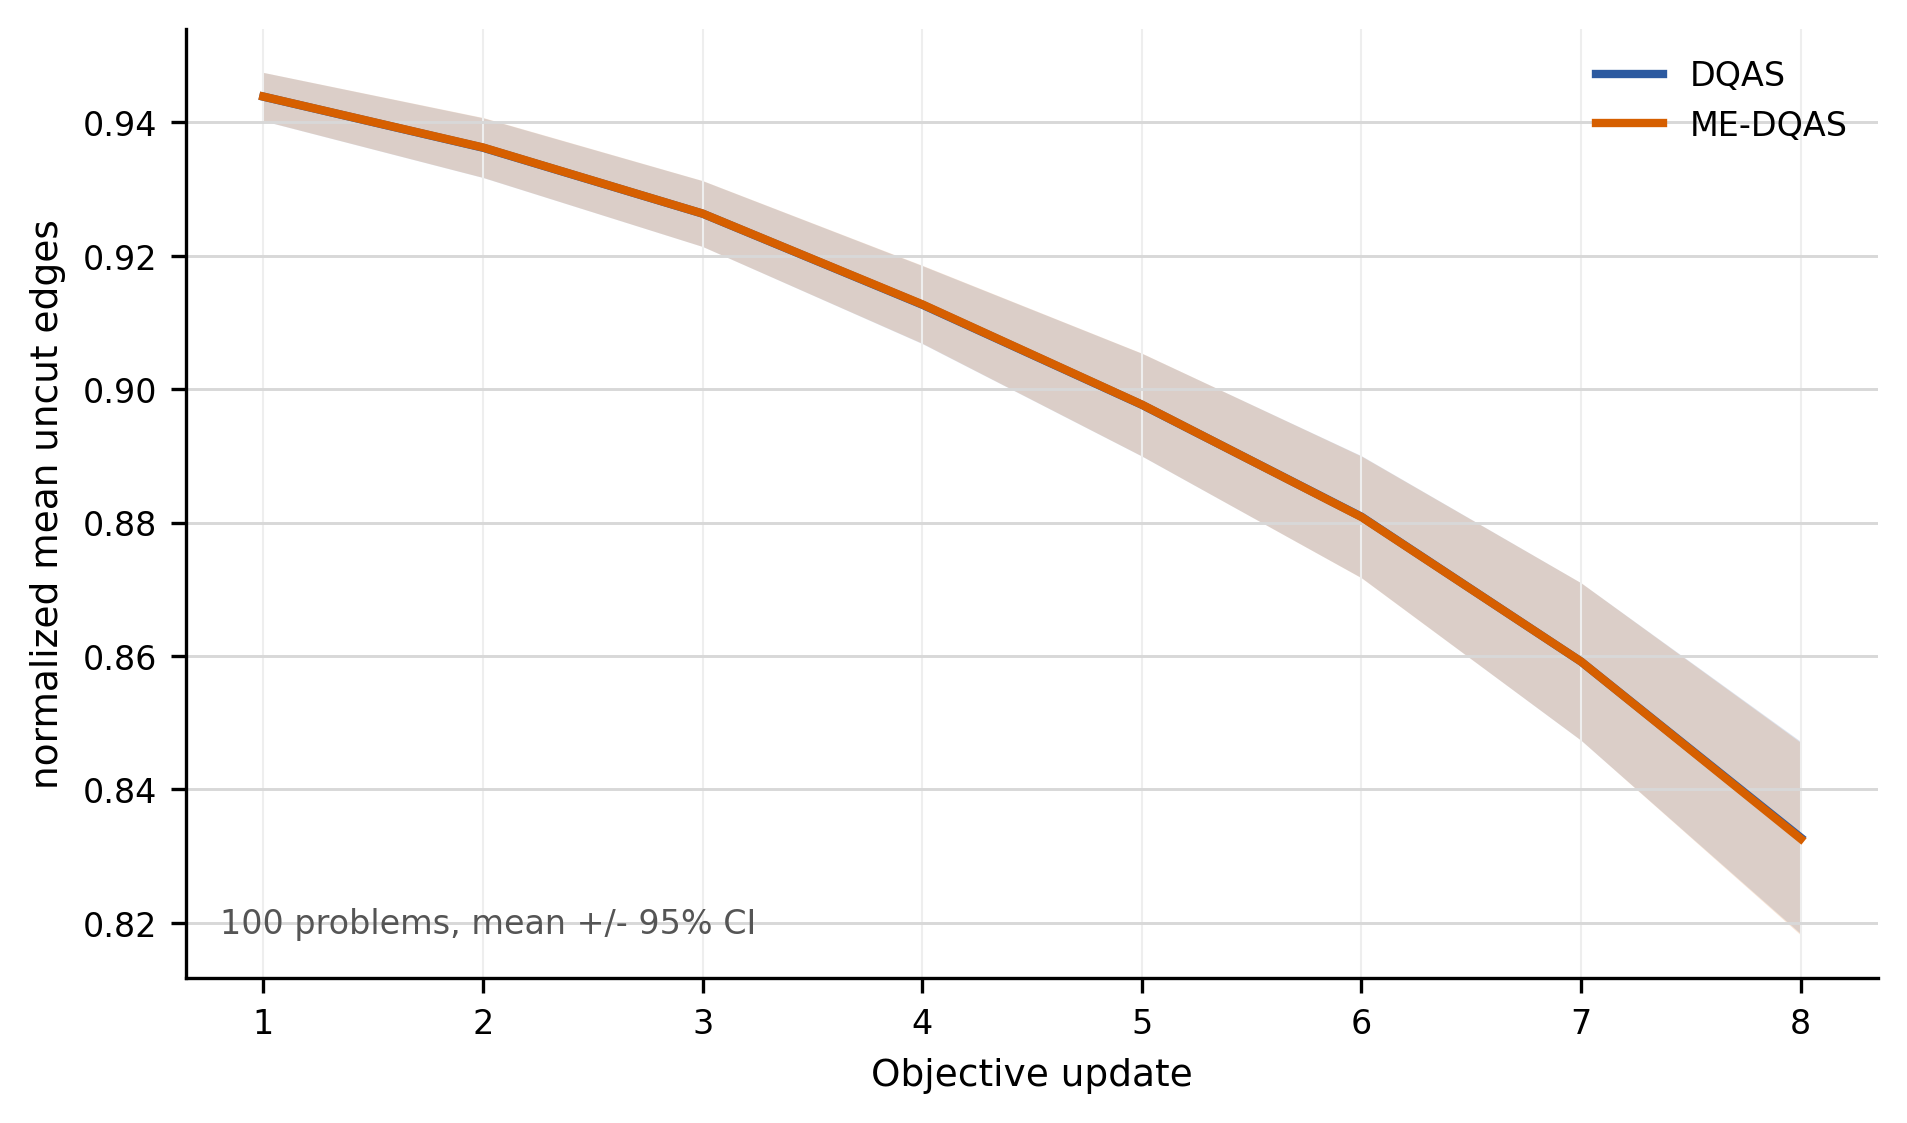
\includegraphics[width=0.84\linewidth]{100_maxcut_search/mean_ci_loss_vs_updates.png}
    \column{0.48\textwidth}\centering
      \uncover<2->{%
        {\small\bfseries Per shot performance}\\[1pt]
        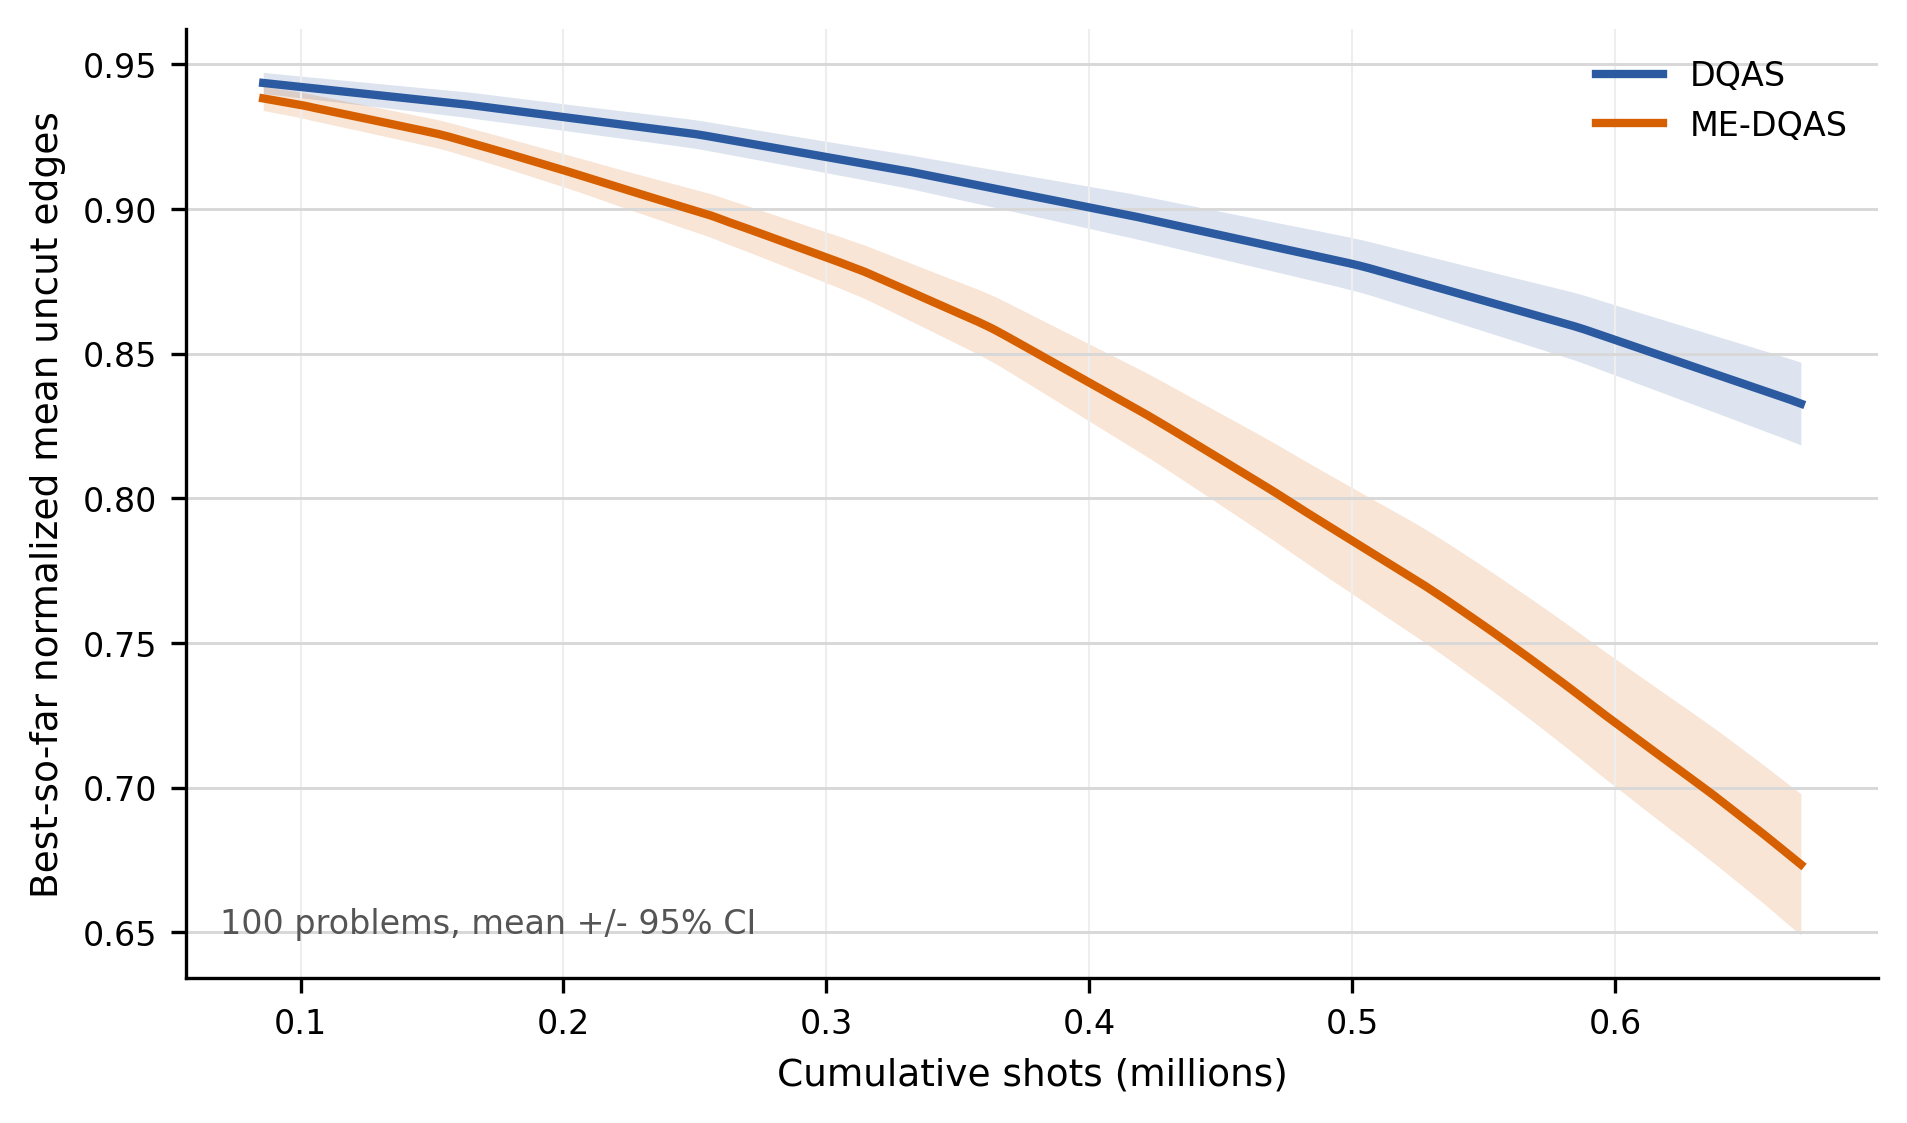
\includegraphics[width=0.84\linewidth]{100_maxcut_search/mean_ci_best_so_far_vs_shots.png}%
      }
  \end{columns}

  \vspace{1.5mm}
  \begin{overlayarea}{\textwidth}{0.65cm}
    \centering
    \only<1>{\normalsize \textbf{Same dynamics per iteration} \;$\Rightarrow$\; curves overlap.}
    \only<2>{\normalsize \textbf{Same 750k budget} \;$\Rightarrow$\; ME-DQAS wins \textcolor{me}{\textbf{200/200}} {\small(3-SAT $0.400\!\to\!0.386$, MaxCut $0.833\!\to\!\textcolor{me}{\mathbf{0.673}}$)}}
  \end{overlayarea}

  \vspace{0.5mm}
  {\scriptsize\color{gray} MaxCut: 100 paired runs, mean $\pm$ 95\% CI (normalized loss: $0$ = exact optimum, $1$ = worst)}
\end{frame}
\note{
[11:05, 1:15] Here is MaxCut (normalized loss: 0 = exact best cut, 1 = worst).
On the left, per optimization update: our rules do \emph{not} change DQAS—exact same dynamics as before, so the two curves overlap pixel for pixel.
(click) Now give both the exact same 750k measurement budget on the right: ME-DQAS pulls away cleanly and outperforms DQAS on all 200 out of 200 paired runs—100/100 on 3-SAT ($0.400 \to 0.386$) and 100/100 on MaxCut ($0.833 \to 0.673$).
}

% ---------------------------------------------------------------- 13 results: where does the performance difference come from?
\begin{frame}{Where does the performance difference come from?}
  \centering
  \vspace{1mm}
  \begin{tikzpicture}
    \begin{axis}[name=cost, width=5.8cm, height=4.4cm, ybar, bar width=13pt, ymin=0, ymax=1.22,
        symbolic x coords={3-SAT,MaxCut}, xtick=data, enlarge x limits=0.48,
        title={\small\bfseries Gradient shots needed (ratio)}, title style={yshift=-2pt},
        ytick={0,0.5,1}, tick label style={font=\footnotesize},
        nodes near coords, every node near coord/.append style={font=\footnotesize},
        nodes near coords style={/pgf/number format/precision=2}]
      \addplot[fill=base!60,draw=none] coordinates {(3-SAT,1.0) (MaxCut,1.0)};
      \addplot[fill=me,draw=none] coordinates {(3-SAT,0.586) (MaxCut,0.606)};
    \end{axis}
    \begin{axis}[name=rounds, at={(cost.east)}, anchor=west, xshift=1.65cm, width=5.8cm, height=4.4cm,
        ybar, bar width=13pt, ymin=0, ymax=17.5,
        symbolic x coords={3-SAT,MaxCut}, xtick=data, enlarge x limits=0.48,
        title={\small\bfseries DQAS rounds in 750k budget}, title style={yshift=-2pt},
        ytick={0,5,10,15}, tick label style={font=\footnotesize},
        nodes near coords, every node near coord/.append style={font=\footnotesize}]
      \addplot[fill=base!60,draw=none] coordinates {(3-SAT,8.99) (MaxCut,8.56)};
      \addplot[fill=me,draw=none] coordinates {(3-SAT,14.05) (MaxCut,13.54)};
    \end{axis}
  \end{tikzpicture}

  \vspace{2.5mm}
  {\normalsize \textcolor{me}{\textbf{41.4\% / 39.4\%}} fewer gradient shots \;$\Rightarrow$\; \textcolor{me}{\textbf{+56\% / +58\%}} more DQAS rounds ($\sim$14 vs.\ $\sim$9)}\\[4pt]
  {\footnotesize\color{softgray} \textcolor{base!80}{$\blacksquare$} DQAS \quad \textcolor{me}{$\blacksquare$} ME-DQAS}
\end{frame}
\note{
[12:20, 1:05] Where does that performance difference come from?
Left: ME-DQAS cuts gradient shots by 41.4\% on 3-SAT and 39.4\% on MaxCut. Right: inside the same 750k budget, those savings buy about 5 extra DQAS rounds—roughly 14 instead of 9 (+56\% / +58\%).
And an honest negative worth sharing: remember our Rule 2 Clifford derivation? With continuous rotation angles, it triggers only 0.05\% of the time on MaxCut and 0.00\% on 3-SAT because angles almost never hit exact $\pi/2$ multiples—which leads directly to an open direction on the next slide!
}

% ---------------------------------------------------------------- 14 actionable
\begin{frame}{Advice for your next project}
  \centering
  \vspace{1.5mm}
  {\huge\bfseries Do you really need to measure that gradient?}\\[5pt]
  {\large\color{me} Before running hardware, check whether it commutes.}

  \vspace{3.5mm}
  \pause
  {\large Works for any shot-based training with a diagonal cost:\\
  QAOA-style circuits, ADAPT-style growth, other architecture search.}

  \vspace{3mm}
  \refs{complementary to Pauli grouping: Verteletskyi+ 2020, Zhao+ 2020, Huang+ 2021}

  \vspace{4mm}
  \pause
  {\normalsize\color{gray} Open: dense / non-diagonal Hamiltonians, hardware noise,\\
  and \textbf{gate pools designed for cheap gradients} (e.g., Clifford-friendly suffixes).}
\end{frame}
\note{
[13:25, 55 s] So on your next variational or architecture search project, ask our title question: do you really need to measure that gradient? Before sending shifted circuits to hardware, run a few lines of classical commutation checks—it is exact and free.
(click) It works for any shot-based training loop with a diagonal cost, and complements Pauli grouping methods.
(click) Open questions: non-diagonal Hamiltonians, hardware noise, and designing gate pools specifically so cheap 0- and 1-circuit (Clifford-friendly) gradients trigger by construction.
}

% ---------------------------------------------------------------- 15 end
\begin{frame}[plain]
  \centering
  \vspace{2mm}
  {\Huge A third of the gradients were zero,\\[3pt] so we just stopped measuring them.}

  \vspace{4mm}
  {\large\bfseries\textcolor{me}{Questions?}\; {\color{navy}Ask now, catch me later, or reach out:}}

  \vspace{4mm}
  \begin{tabular}{cc}
    \qrcode[height=2.05cm]{https://arxiv.org/abs/2610.10351} & \qrcode[height=2.05cm]{https://github.com/Newida/ME-DQAS}\\[2pt]
    \small arXiv:2610.10351 & \small github.com/Newida/ME-DQAS
  \end{tabular}

  \vspace{4mm}
  {\small \textbf{Lukas Theißinger} \quad\textperiodcentered\quad \texttt{lukas.theissinger@uni-bonn.de}}\\[2.5pt]
  {\footnotesize\color{softgray} \textbf{LinkedIn:} \texttt{linkedin.com/in/lukas-theißinger}}
\end{frame}
\note{
[14:20 -> 14:30, then 5 min Q\&A] Thank you! Paper, code, and all 200 paired runs are behind the QR codes—happy to take your questions now!
}

\end{document}
